% ======================= Pre-Amble =========================
      
%Format
\documentclass[11pt, oneside]{article}   	% use "amsart" instead of "article" for AMSLaTeX format 
                     						%imports package {article} and specify option(s) [11pt, oneside]
\usepackage{geometry}                		% See geometry.pdf to learn the layout options. There are lots. 
    \geometry{letterpaper}                   		% ... or a4paper or a5paper or ... 
    %\geometry{landscape}                		% Activate for rotated page geometry

\usepackage[parfill]{parskip}    		        % Activate to begin paragraphs with an empty line rather than an indent

    %Colours
    \usepackage{graphicx, subcaption}
    \usepackage[usenames, dvipsnames]{color}     % font colour:    \textcolor{<colour>}{text}
          									%highlight text:  \colorbox{<color>}{text}
    \usepackage{soul}						%highlight text: \hl{}     %only  yellow								
    									%list of colours: https://www.sharelatex.com/learn/Using_colours_in_LaTeX
    									
    %Bullets
    \usepackage{enumerate}     %specify type of enumeration: \being{enumerate}[<type of enumeration>]
    
    %Footnote Spacing
    \setlength{\footnotesep}{0.4cm}                  %specify spacing b/w footnotes
    \setlength{\skip\footins}{0.6cm}                    % space b/w footnotes and textbody


%Mattematics
    %American Mathematics Society packages
    \usepackage{amsmath}	   %math
    \usepackage{amssymb}       %symbols
    \usepackage{amsthm}          %theorems

    %QED
    \newcommand*{\QEDA}{\hfill\ensuremath{\blacksquare}}         %make qed filled square:    \QEDA
    \newcommand*{\QEDB}{\hfill\ensuremath{\square}}               %make qed empty square: \QEDB 
    
    \renewcommand\qedsymbol{\ensuremath{\blacksquare}}		%Proof environment


%Figures
\usepackage{caption}
\captionsetup[figure]{labelfont=bf}    %make figure labels boldface
\captionsetup[table]{labelfont=bf}     %make table labels boldface

\usepackage[hidelinks]{hyperref}                % Allows for clickable references

    %Tables
    \usepackage[none]{hyphenat}                    % Stops breaking-up words in a table (i.e. no hyphens)                                                             
    
    \usepackage{array}   
        \newcolumntype{x}[1]{>{\centering\let\newline\\\arraybackslash\hspace{0pt}}p{#1}}       %center fixed column width: x{<len>}                      
        \newcolumntype{$}{>{\global\let\currentrowstyle\relax}}                                                   % let us apply things (e.g. bold/italicize) to entire row            
        \newcolumntype{^}{>{\currentrowstyle}}
        \newcommand{\rowstyle}[1]{\gdef\currentrowstyle{#1} #1\ignorespaces}
    
    %Images
    \graphicspath{ {images/} }                          %directory that your images are located in within your current directory
    
    %Diagrams
    \usepackage[latin1]{inputenc}
    \usepackage{tikz}
    	\tikzset{line/.style={-latex'}}
        \usepackage{tkz-berge}
        \usetikzlibrary{shapes,arrows}
        \usetikzlibrary{patterns}			%Specify colours of stuff (e.g. vertices): 
        								%	-> set style: \tikzset{VertexStyle/.append style = {minimum size = 8pt, inner sep = 0pt}} 
								%	-> change individual vertices: \AddVertexColor{white}{1,2} 


%Bibliography
\usepackage[numbers,sort&compress]{natbib}   %for multiple references: sorts  (i.e. [1,2] NOT [2, 1] )
                                           				  %                                     compresses (i.e. [1-3] )
\usepackage[nottoc]{tocbibind}                            %add bibliography to table of contents


%Miscellaneous
\usepackage{dirtytalk}    %quotations: use \say  


%================== Header & Footer =========================
\usepackage{fancyhdr}
\usepackage{lastpage}      %ensures you can reference LastPage (i.e. Page 2 of 10)

\renewcommand{\headrulewidth}{0.4pt}		%Decorative Header line: thickness={0.4pt}
\renewcommand{\footrulewidth}{0.4pt}		%Decorative Footer line: thickness={0.4pt}

\setlength{\headheight}{13.6pt} 		%space b/w top of page & header
\setlength{\headsep}{0.3in}		%space b/w page header and body

%Make Header & Footer    
\pagestyle{fancy}
    \lhead{Stephanie Knill} 		% controls the left corner of the header
    \chead{} 					% controls the center of the header
    \rhead{} 					% controls the right corner of the header
    \lfoot{} 					% controls the left corner of the footer
    \cfoot{Page~\thepage\ of \pageref{LastPage}} 				% controls the center of the footer
    												%Page~\thepage\  if just want Page x
    \rfoot{}			 		% controls the right corner of the footer

% =============================== Document ===================================
\begin{document}

% Title Page
\title{MATH 442 --- Assignment 10 \\
\line(1,0){360} \\              %(slope x, y){length of line}
}
\author{
Stephanie Knill \\
54882113 \\
Due: March 24, 2016}

\date{}                   % Activate:  display a given date (e.g. {August 4} ) or no date (empty {} )
                                    %No activate: display current date
\maketitle

%\thispagestyle{empty}                   %Remove header from this (first) page. Change empty -> plain to keep numbering
%								-> Doesn't matter in this case (b/c title page)
%\cleardoublepage


% ================= Questions ================

\section*{Question 55}

If $G$ is a simple connected graph, then for any edge in $e$ in $G$
\begin{align}
\tau(G) = \tau(G-e) + \tau(G/e)
\label{eq1}
\end{align}

\begin{proof}
\hl{no ducking clue}
\end{proof}

\section*{Question 51}

For the graph $G$ of vertices $v_1, v_2, \ldots v_5$ in Figure \ref{Graph1}, let us determine the number of non-isomorphic ways to label it. Here, we can label $v_1$ 5 different ways. For the vertex pair $v_2$ and $v_5$, we can label them ${4 \choose 2}=6$ ways, Lastly we can label $v_3$ 2 different ways (due to isomorphism, $v_4$ simply takes the remaining label). This gives us a total of
$$5 \cdot 6 \cdot 2 = 60$$
non-isomorphic ways to label graph $G$.
\begin{figure}[h]           
            \centering
            \begin{subfigure}[b]{0.45\columnwidth}
            	\centering
             	 \begin{tikzpicture}[scale=0.75,transform shape]
        		
        		\GraphInit[vstyle=Classic]					%Make vertice labels outside it
        		%\SetVertexNoLabel							%No vertice labels
        		\tikzset{VertexStyle/.append style = {fill=black, circle}}		%Set vertex style        		
			\Vertex [x=0,y=0, L= $v_3$]{1}
			\Vertex [x=3, y=0, L=$v_4$]{2}
			\Vertex [x=3, y=3, L=$v_5$]{3}
			\Vertex [x=0, y=3, L=$v_2$]{4}
			\Vertex [x=1.5, y=5,L=$v_1$]{5}
        		%\AddVertexColor{white}{1,2} 					%Change individual vertex type
            
        			\path [thick] (1) edge (2);			%arrows: [line];     label: {$label}$
			\path [thick] (2) edge (3);
			\path [thick] (3) edge (4);
			\path [thick] (1) edge (4);
			\path [thick] (3) edge (5);
			\path [thick] (4) edge (5);
            	\end{tikzpicture}
            	\caption{Graph $G$}
		\label{Graph1}
            \end{subfigure}
           \begin{subfigure}[b]{0.45\columnwidth}
            	\centering
             	 \begin{tikzpicture}[scale=0.75,transform shape]
        		
        		\GraphInit[vstyle=Classic]					%Make vertice labels outside it
        		%\SetVertexNoLabel							%No vertice labels
        		\tikzset{VertexStyle/.append style = {rectangle}}		%Set vertex style        		
			\Vertex [x=0,y=0, L=$v_2$]{2}
			\Vertex [x=2, y=0, L=$v_3$]{3}
			\Vertex [x=4, y=0, L=$v_4$]{4}
			\Vertex [x=2, y=3, L=$v_5$]{5}
			\Vertex [x=2, y=-3, L=$v_1$]{1}
        		%\AddVertexColor{white}{1,2} 					%Change individual vertex type
            
        			\path [thick] (1) edge (3);			%arrows: [line];     label: {$label}$
			\path [thick] (2) edge (3);
			\path [thick] (3) edge (4);
			\path [thick] (2) edge (5);
			\path [thick] (3) edge (5);
			\path [thick] (4) edge (5);

            	\end{tikzpicture}
            	\caption{Graph $H$}
		\label{Graph2}
            \end{subfigure}
           
            \caption{Graphs $G$ and $H$.}
            \label{polynomials}
        \end{figure}
For the graph $H$ of vertices $v_1, v_2, \ldots v_5$ in Figure \ref{Graph2}, we can label $v_1$ 5 ways, $v_3$ 4 ways, and $v_5$ 3 ways. Since $v_2$ and $v_4$ are symmetrical about the y-axis (i.e. same degree), then labelling them the remaining labels does not create any new non-isomorphic graphs. This gives us a total of
$$5 \cdot 4 \cdot 3 = 60$$
non-isomorphic ways to label graph $H$.


\section*{Question 57}

\begin{enumerate}[\quad (a)]
	\item For the labelled graph (Figure \ref{q57a}), the associate Pr\"{u}fer sequence is (5,2,2,6,2,2).
	\begin{figure}[h]
	\centering
        \begin{tikzpicture}[scale=0.75,transform shape]
		
		%\GraphInit[vstyle=Classic]					%Make vertice labels outside it
		%\SetVertexNoLabel							%No vertice labels
		\tikzset{VertexStyle/.append style = {circle}}		%Set vertex style
			%\AddVertexColor{white}{1,2} 					%Change individual vertex type
			\Vertex [x=0,y=0]{8}
			\Vertex [x=2, y=0]{4}
			\Vertex [x=4, y=0]{7}
			\Vertex [x=2, y=2]{2}
			\Vertex [x=4, y=2]{3}
			\Vertex [x=2, y=5]{6}
			\Vertex [x=6, y=5]{5}
			\Vertex [x=8, y=3]{1}
    		
		\path [solid] (2) edge (8);					%arrows: [line];     label: {$label}$
		\path [solid] (2) edge (4);	
		\path [solid] (2) edge (7);	
		\path [solid] (2) edge (3);	
		\path [solid] (2) edge (6);	
		\path [solid] (6) edge (5);	
		\path [solid] (5) edge (1);		
    	\end{tikzpicture}  
        \caption{Labelled graph $G$ with associated Pr\"{u}fer sequence (5,2,2,6,2,2).}
        \label{q57a}
	\end{figure}
	
 	\item For the Pr\"{u}fer sequence (3,4,8,1,8,8,8), the associated labelled graph $H$ can be seen in Figure \ref{q57b}.
	\begin{figure}[h]
	\centering
	\begin{tikzpicture}[scale=0.75,transform shape]	
		%\GraphInit[vstyle=Classic]					%Make vertice labels outside it
		%\SetVertexNoLabel							%No vertice labels
		\tikzset{VertexStyle/.append style = {circle}}		%Set vertex style
			%\AddVertexColor{white}{1,2} 					%Change individual vertex type
			\Vertex [x=0,y=0]{2}
			\Vertex [x=2, y=0]{3}
			\Vertex [x=4, y=0]{4}
			\Vertex [x=6, y=0]{8}
			\Vertex [x=8, y=0]{1}
			\Vertex [x=10, y=0]{5}
			\Vertex [x=4, y=-2]{6}
			\Vertex [x=6, y=-2]{7}
			\Vertex [x=8, y=-2]{9}
    		
		\path [solid] (2) edge (3);					%arrows: [line];     label: {$label}$
		\path [solid] (3) edge (4);	
		\path [solid] (4) edge (8);	
		\path [solid] (8) edge (1);	
		\path [solid] (1) edge (5);	
		\path [solid] (8) edge (6);	
		\path [solid] (8) edge (7);	
		\path [solid] (8) edge (9);		
    	\end{tikzpicture}  
        \caption{Labelled graph $H$ with associated Pr\"{u}fer sequence (3,4,8,1,8,8,8).}
        \label{q57b}
	\end{figure}
\end{enumerate}


\section*{Question 58}

A vertex in a labelled graph has degree $k$ if and only if its label appears $k-1$ times in the Pr\"{u}fer sequence of the graph.
\begin{proof}
$\Rightarrow$ Assume that a vertex $v$ in a labeled graph has degree $k$. Here, we take a leaf and put its adjacent vertex in the Pr\"{u}fer sequence and then delete that leaf. We have two cases for our vertex $v$ of degree $k$

\emph{Case 1:} $v$ is a leaf. Then it is never in the Pr\"{u}fer sequence. Here $k=deg(v)=1$ and the number of occurrences is $k-1= 0$.

\emph{Case 2:} $v$ is a non-leaf. We add it to the Pr\"{u}fer sequence and minus its degree by 1. This continues until either it is a leaf (deleted) or it is one of the last two leaves (do not add to Pr\"{u}fer sequence). Either way, it is only added to the Pr\"{u}fer sequence $k-1$ times. 

$\Leftarrow$ Assume that a vertex label appears $k-1$ times in Pr\"{u}fer sequence of a graph. Then this vertex label was a non-leaf adjacent to a deleted leaf $k-1$ times until it became a leaf itself. Thus it had original degree $(k-1)+1 = k$.
\end{proof}

\section*{Question 59}

There does not exist a tree consisting of 12 vertices, with one vertex of degree 5, two vertices of degree 4, and one vertex of degree 2.

\begin{proof}
Assume to the contrary that such a graph exists. Since we cannot form cycles, let us connect these four vertices of degree 5, 5, 5, and 2 together. Without loss of generality, let us attach the vertices of degree 4 and 2 to the vertex of degree 5 (Figure \ref{q59}).
\begin{figure}[h]
	\centering
	\begin{tikzpicture}[scale=0.75,transform shape]	
		%\GraphInit[vstyle=Classic]					%Make vertice labels outside it
		%\SetVertexNoLabel							%No vertice labels
		\tikzset{VertexStyle/.append style = {circle}}		%Set vertex style
			%\AddVertexColor{white}{1,2} 					%Change individual vertex type					
			\Vertex [x=0,y=0]{5}
			\Vertex [x=8, y=0]{11}
			\Vertex [x=2, y=2]{6}
			\Vertex [x=1, y=-2]{7}
			\Vertex [x=3, y=-2]{9}
			\Vertex [x=5, y=-4]{13}
			\Vertex [x=4, y=2]{8}
			\Vertex [x=6, y=2]{10}
			\Vertex [x=7, y=-2]{12}
			
			\tikzset{VertexStyle/.append style = {fill=pink, circle}}
			\Vertex [x=2, y=0]{1}
			\Vertex [x=4, y=0]{2}
			\Vertex [x=6, y=0]{3}
			\Vertex [x=5, y=-2]{4}

    		
		\path [solid] (5) edge (1);					%arrows: [line];     label: {$label}$
		\path [solid] (1) edge (2);	
		\path [solid] (2) edge (3);	
		\path [solid] (3) edge (11);	
		\path [solid] (1) edge (6);	
		\path [solid] (1) edge (7);	
		\path [solid] (2) edge (8);	
		\path [solid] (2) edge (9);
		\path [solid] (2) edge (4);		
		\path [solid] (4) edge (13);
		\path [solid] (3) edge (10);
		\path [solid] (3) edge (12);
    	\end{tikzpicture}  
        \caption{Graph of tree $T$ with vertices $v_1$ and $v_3$ of degree 4, $v_2$ of degree 5, and $v_4$ of degree 2 (denoted by pink).}
        \label{q59}
	\end{figure}
	
Since this is a tree, none of the edges from these four vertices can connect back to $v_1, v_2, v_3$ or $v_4$. Thus we must attach a new vertex on the ends of each of them. However we have 9 edges which will result in a total of 13 vertices in $T$, thereby giving us the necessary contradiction.
\end{proof}

\cleardoublepage

\section*{Question 60}

\emph{How many labelled trees exist with 6 vertices such that the degree of ever vertex is 1 or 3?}

Since we can only have vertices of degree 1 or 3, this gives us one possible configuration: two vertices of degree 3 attached with vertices of degree 1 on the remaining edges (Figure \ref{q60}). If we were to have less vertices of degree 3---in this case, zero or one---we will have less than 6 vertices total. If we were to have greater than two vertices of degree 3, we will have more than 6 vertices. Thus we can only have a configuration with exactly two vertices of degree 3.

\begin{figure}[h]
	\centering
	\begin{tikzpicture}[scale=0.75,transform shape]	
		%\GraphInit[vstyle=Classic]					%Make vertice labels outside it
		\SetVertexNoLabel							%No vertice labels
		\tikzset{VertexStyle/.append style = {fill=black, circle}}		%Set vertex style
			%\AddVertexColor{white}{1,2} 					%Change individual vertex type					
			\Vertex [x=0,y=0]{1}
			\Vertex [x=3, y=0]{2}
			\Vertex [x=-2, y=2]{3}
			\Vertex [x=-2, y=-2]{4}
			\Vertex [x=5, y=2]{5}
			\Vertex [x=5, y=-2]{6}
    		
		\path [solid] (1) edge (2);					%arrows: [line];     label: {$label}$
		\path [solid] (1) edge (3);
		\path [solid] (1) edge (4);
		\path [solid] (2) edge (5);
		\path [solid] (2) edge (6);	
    	\end{tikzpicture}  
        \caption{Graph of 6 vertices with vertices of degree 1 or 3.}
        \label{q60}
	\end{figure}
	
Let us first fix the labels of the vertices of degree 1. Since we can rotate about the vertices of degree 3 and flip the graph about its line of symmetry in the $y$-axis, two graphs are isomorphic if they have the same labels attached to a vertex of degree 3. Let the possible labels be 1, 2, 3, and 4. Then for labels $i,j$, where $i\neq j$ and $i,j \in \{1,2,3,4\}$, we must assign each $i$ and $j$ such that they are adjacent to the same vertex of degree 3 and adjacent to different vertices of degree 3. This gives us 3 possible configurations (Figure \ref{q60}) for the fixing of the labels for vertices of degree 1.

 \begin{figure}[h]
    \centering
    
    \begin{subfigure}[b]{0.3\columnwidth}             
    \centering
      \begin{tikzpicture}[scale=0.6,transform shape]
			\Vertex [x=-2, y=2,L=1]{3}
			\Vertex [x=-2, y=-2,L=2]{4}
			\Vertex [x=4, y=2,L=3]{5}
			\Vertex [x=4, y=-2,L=4]{6}
			\SetVertexNoLabel	
			\Vertex [x=0,y=0]{1}
			\Vertex [x=2, y=0]{2}
    		
		\path [solid] (1) edge (2);					%arrows: [line];     label: {$label}$
		\path [solid] (1) edge (3);
		\path [solid] (1) edge (4);
		\path [solid] (2) edge (5);
		\path [solid] (2) edge (6);
      \end{tikzpicture}
      \caption{Configuration 1}
      \label{A}
    \end{subfigure}
    \begin{subfigure}[b]{0.3\columnwidth}
      \centering
      \begin{tikzpicture}[scale=0.6,transform shape]
			\Vertex [x=-2, y=2,L=1]{3}
			\Vertex [x=-2, y=-2,L=3]{4}
			\Vertex [x=4, y=2,L=2]{5}
			\Vertex [x=4, y=-2,L=4]{6}
			\SetVertexNoLabel	
			\Vertex [x=0,y=0]{1}
			\Vertex [x=2, y=0]{2}
    		
		\path [solid] (1) edge (2);					%arrows: [line];     label: {$label}$
		\path [solid] (1) edge (3);
		\path [solid] (1) edge (4);
		\path [solid] (2) edge (5);
		\path [solid] (2) edge (6);
      \end{tikzpicture}
      \caption{Configuration 2}
    \end{subfigure}
    \begin{subfigure}[b]{0.3\columnwidth}
      \centering
      \begin{tikzpicture}[scale=0.6,transform shape]
			\Vertex [x=-2, y=2,L=1]{3}
			\Vertex [x=-2, y=-2,L=4]{4}
			\Vertex [x=4, y=2,L=2]{5}
			\Vertex [x=4, y=-2,L=3]{6}
			\SetVertexNoLabel	
			\Vertex [x=0,y=0]{1}
			\Vertex [x=2, y=0]{2}
    		
		\path [solid] (1) edge (2);					%arrows: [line];     label: {$label}$
		\path [solid] (1) edge (3);
		\path [solid] (1) edge (4);
		\path [solid] (2) edge (5);
		\path [solid] (2) edge (6);
    	\end{tikzpicture}
    	\caption{Configuration 3}
    \end{subfigure}
    \caption{Possible configurations for the fixing of the labels for vertices of degree 1.}
    \label{q60}
    \end{figure}

Now, let us fix the labels for the two vertices of degree 3. Although we have a line of symmetry about the y-axis along the edge adjacent to our two vertices of degree 3, switching the assigned labels for these vertices will yield non-isomorphic graphs (Figure \ref{q60 swap}). Thus for each of the remaining labels, we have 2 possible arrangements.

 \begin{figure}[h]
    \centering
    
    \begin{subfigure}[b]{0.4\columnwidth}             
    \centering
      \begin{tikzpicture}[scale=0.7,transform shape]
			\Vertex [x=-2, y=2,L=1]{3}
			\Vertex [x=-2, y=-2,L=2]{4}
			\Vertex [x=4, y=2,L=3]{5}
			\Vertex [x=4, y=-2,L=4]{6}	
			\Vertex [x=0,y=0,L=5]{1}
			\Vertex [x=2, y=0,L=6]{2}
    		
		\path [solid] (1) edge (2);					%arrows: [line];     label: {$label}$
		\path [solid] (1) edge (3);
		\path [solid] (1) edge (4);
		\path [solid] (2) edge (5);
		\path [solid] (2) edge (6);
      \end{tikzpicture}
      \caption{Configuration 1}
      \label{A}
    \end{subfigure}
    \begin{subfigure}[b]{0.4\columnwidth}
      \centering
      \begin{tikzpicture}[scale=0.7,transform shape]
			\Vertex [x=-2, y=2,L=1]{3}
			\Vertex [x=-2, y=-2,L=2]{4}
			\Vertex [x=4, y=2,L=3]{5}
			\Vertex [x=4, y=-2,L=4]{6}
			\Vertex [x=0,y=0,L=6]{1}
			\Vertex [x=2, y=0,L=5]{2}
    		
		\path [solid] (1) edge (2);					%arrows: [line];     label: {$label}$
		\path [solid] (1) edge (3);
		\path [solid] (1) edge (4);
		\path [solid] (2) edge (5);
		\path [solid] (2) edge (6);
      \end{tikzpicture}
      \caption{Configuration 2}
    \end{subfigure}
    \caption{Swapping labels for the vertices of degree 3 yields non-isomorphic graphs.}
    \label{q60 swap}
    \end{figure}

However,  for the remaining vertices we have 6 different labels for which we must choose 2. This gives us ${6 \choose 2}=15$ possibilities. Multiplying all of these togethers gives us a total of
$$3 \cdot 2 \cdot 15 = 90$$
non-isomorprhic labelled trees with 6 vertices of degree 1 or 3.



\end{document} 